% Schema der Glattalbahn-Verlängerung nach Kloten (eigene Darstellung, nicht massstäblich).
% Ersetzt die frühere Projektkarte GTB_Karte_mit_Legende_Web_v02.png (keine freie Lizenz belegt).
% Verwendet in Slides/K06dListenTeil2.tex und Exam_Questions/QuestionsProg.tex.
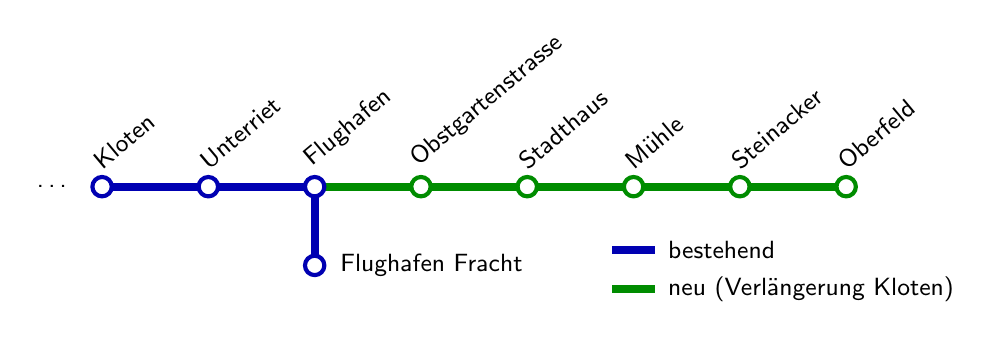
\begin{tikzpicture}[x=1.35cm, font=\sffamily\small,
		station/.style={circle, draw=#1, fill=white, line width=1.5pt, minimum size=7pt, inner sep=0pt},
		name/.style={anchor=south west, rotate=40, inner sep=1pt}]
	% bestehende Strecke (blau) bis Flughafen, Abzweigung nach Flughafen Fracht
	\draw[line width=3pt, blue!70!black] (0,0) -- (2,0);
	\draw[line width=3pt, blue!70!black] (2,0) -- (2,-1);
	% neue Strecke (grün)
	\draw[line width=3pt, green!55!black] (2,0) -- (7,0);
	\foreach \x/\name/\farbe in {
			0/Kloten/blue!70!black, 1/Unterriet/blue!70!black, 2/Flughafen/blue!70!black,
			3/Obstgartenstrasse/green!55!black, 4/Stadthaus/green!55!black, 5/Mühle/green!55!black,
			6/Steinacker/green!55!black, 7/Oberfeld/green!55!black} {
			\node[station=\farbe] at (\x,0) {};
			\node[name] at (\x,.15) {\name};
		}
	\node[station=blue!70!black] at (2,-1) {};
	\node[anchor=west] at (2.15,-1) {Flughafen Fracht};
	\node[anchor=east] at (-.2,0) {\ldots};
	% Legende
	\draw[line width=3pt, blue!70!black] (4.8,-.8) -- (5.2,-.8) node[right, black] {bestehend};
	\draw[line width=3pt, green!55!black] (4.8,-1.3) -- (5.2,-1.3) node[right, black] {neu (Verlängerung Kloten)};
\end{tikzpicture}
